\documentclass[../main.tex]{subfiles}

\begin{document}
	
	В данном разделе приведены схемы алгонитмов:
	\begin{enumerate}[1)]
		\item Кнута-Морриса-Пратта
		\item Бойера Мура
	\end{enumerate}

	\begin{figure}[H]
		\centering
		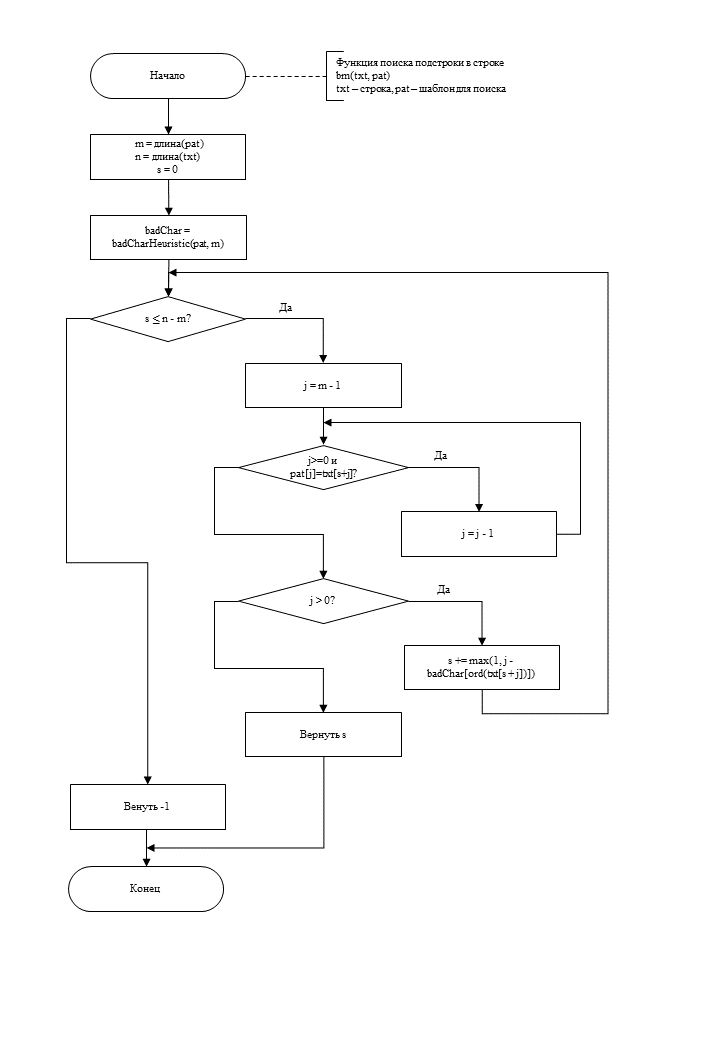
\includegraphics[scale=0.7 ]{src/img/bm-main}
		\caption{}
		\label{fig:bm-main}
	\end{figure}
	
	\begin{figure}[H]
		\centering
		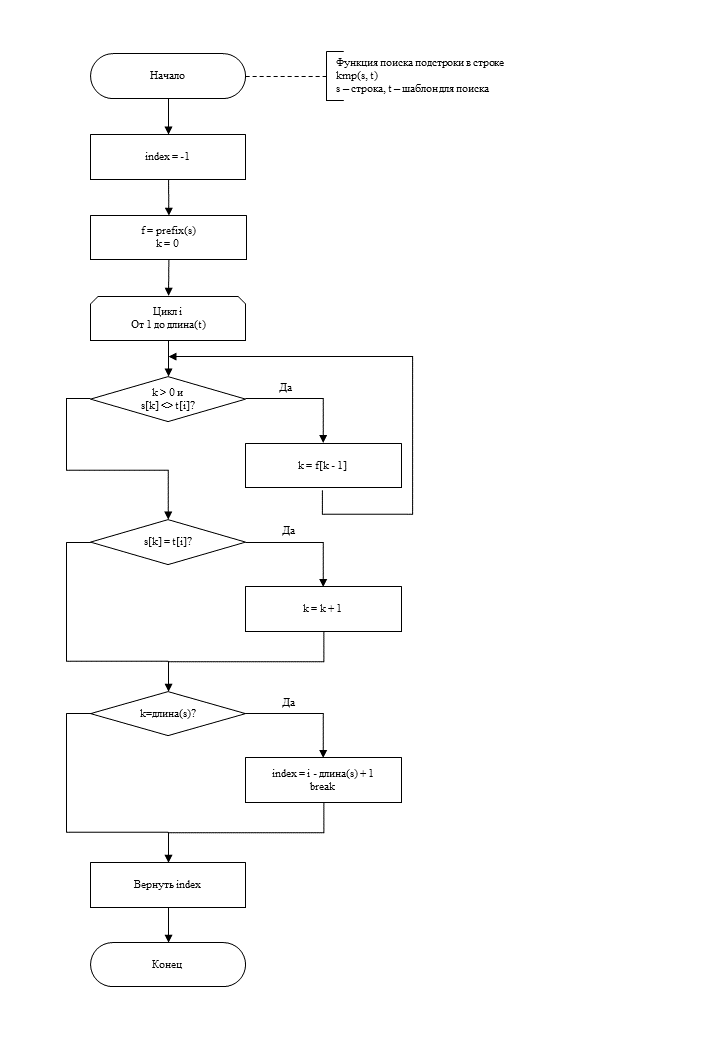
\includegraphics[scale=0.7 ]{src/img/kmp-main}
		\caption{}
		\label{fig:kmp-main}
	\end{figure}
	
	\begin{figure}[H]
		\centering
		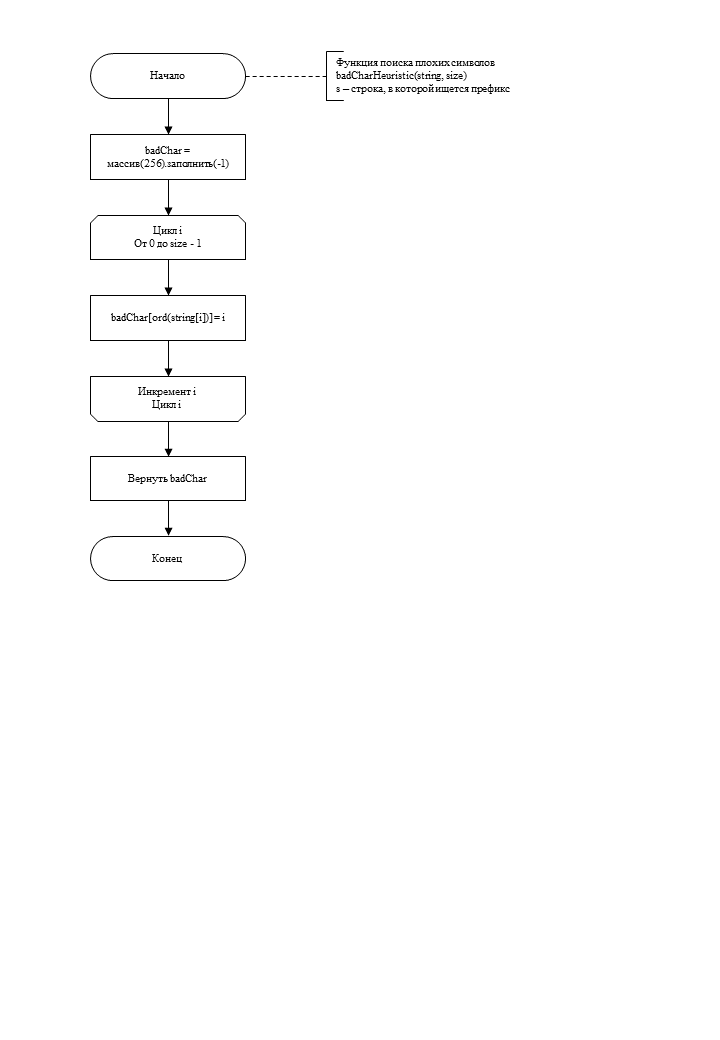
\includegraphics[scale=0.7 ]{src/img/bm-prepare}
		\caption{}
		\label{fig:bm-prepare}
	\end{figure}
	
	\begin{figure}[H]
		\centering
		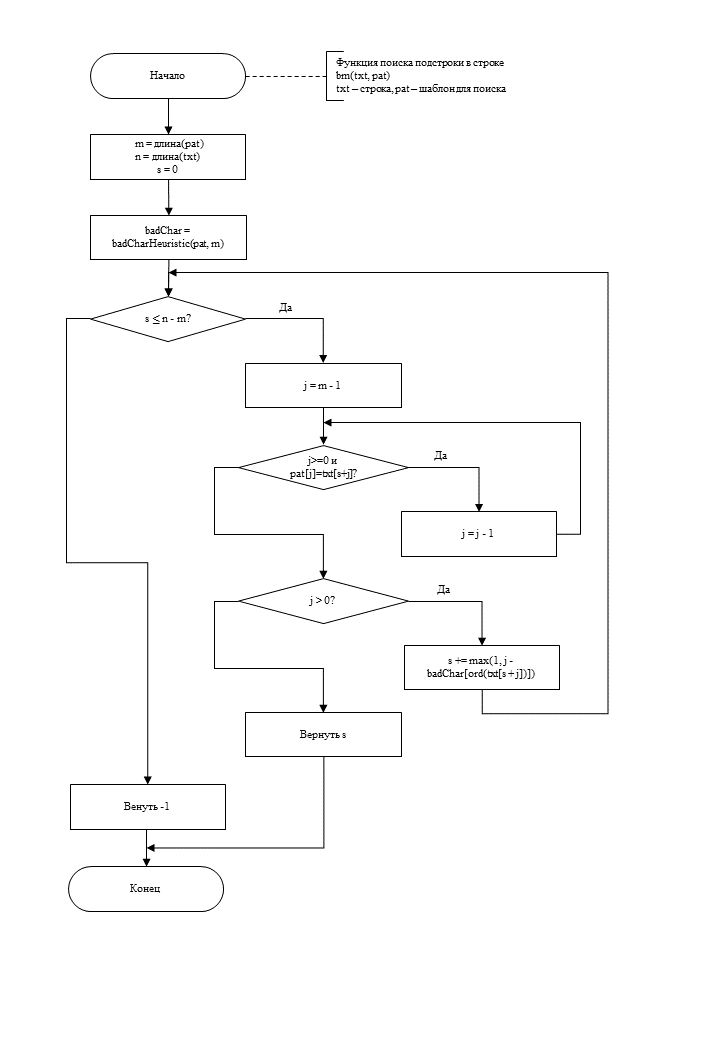
\includegraphics[scale=0.7]{src/img/bm-main}
		\caption{}
		\label{fig:bm-main}
	\end{figure}
	
	В данном разделе были приведены схемы алгоритмов поиска подстроки в строке Кнута-Морриса-Пратта и Бойера Мура
	
\end{document}